\newpage
\section{Brand identity}
\label{sec:brand}

Brand identity is the visible elements of a brand, such as color, design, and logo, that identify and distinguish the brand in consumers' minds. Brand identity is distinct from brand image.\cite{brand-identity}

In this section, I'm going to explain the process and decisions taken in order to design a solid brand identity.

\subsection{Color Palette}

When choosing a brand's color it's useful to define the concepts we want to relate to the brand. In this case, GradeCalc is related to: \textit{grades}, \textit{exam}, \textit{school}, \textit{math}, \textit{study}... And we want to communicate: \textit{success}, \textit{hope}, \textit{intelligence} and sometimes \textit{failure}.

The most representative colors of grades are green and red because they represent the correctness of an answer. Where green means \textit{right} and red means \textit{wrong}. So, these two colors must be indubitably present in the app. 
% Other relevant colors are blue, yellow, and gray, all of them are considered to represent \textit{intelligence}, and intelligence is what grades evaluate.

\vfill
\begin{figure}[ht!]
    \center
    \includegraphics[width=0.3333\columnwidth]{media/color-palette-wheel.png}
    \caption{GradeCalc's colors in the color wheel}
    \label{fig:color-palette-wheel}
\end{figure}
\vfill

\newpage
Because we want to communicate success over failure, green is GradeCalc's primary color. And red is going to be used to convey warning and failure, as usual in interfaces, but due to the nature of this app it's going to be more present than usual, and this is why it's the app's tertiary color.

Red and green are complementary\footnote{Two colors are \textbf{complementary} when they are opposite each other on the color wheel.} colors, so if we want to add another one to the palette using color theory\cite{color-harmonies}, the only option is to use a tetradic color combination, ether rectangular\footnote{A \textbf{rectangular tetradic} color scheme has four colors arranged into two complementary pairs.} or square\footnote{In a \textbf{square tetradic} color scheme all four colors spaced evenly around the color circle.}. Using a square tetradic scheme gives us blue or orange (Fig. \ref{fig:color-palette-wheel}), I chose blue because it's less vibrant and can be used easier as a compliment.

Finally, the background is white, and the text dark gray. I chose this combination because it recalls a paper written with a pencil. This is the final color palette (Fig. \ref{fig:color-palette}):

\vfill
\begin{figure}[ht!]
    \center
    \vspace*{-0.25in}
    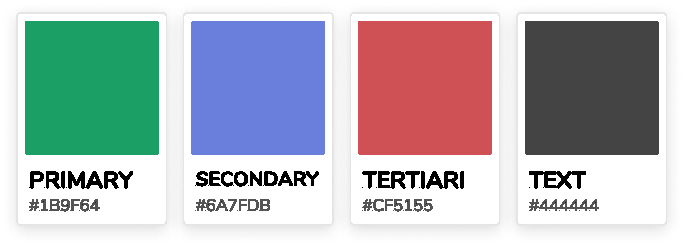
\includegraphics[scale=1.25]{media/color-palette.pdf}
    \vspace*{-0.125in}
    \caption{GradeCalc's color palette}
    \label{fig:color-palette}
\end{figure}
\vfill
\begin{figure}[ht!]
    \center
    \vspace*{-0.5in}
    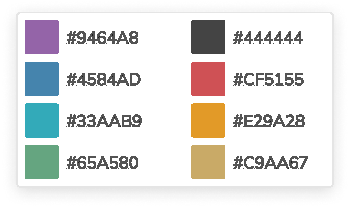
\includegraphics[scale=1.25]{media/color-palete-subjects.pdf}
    \vspace*{-0.125in}
    \caption{GradeCalc's subject's colors}
    \label{fig:color-palette-subjects}
\end{figure}
\vspace*{-0.5in}´
\vfill

\newpage
\subsection{Typography}

Nunito is an open-source typeface created by Vernon Adams. Its a rounded terminal sans-serif font for display but there's also a non-rounded terminal version.

Nunito is a well balanced, highly-readable sans-serif typeface. The characters have thin, uniform stroke widths that work well for both body and display copy. The project began as a rounded terminal sans-serif for display typography, before being extended to a terminal version.\cite{nunito-pairing}

I chose Nunito because it's roundness makes it resembles slightly a handwritten typeface. In exams, the grades are always handwritten, and using this typography makes the grades in the app look like the ones in paper, but with highly-readability. 

Another reason for choosing Nunito is that it pairs well with itself, allowing it to be the only font in the app.

\vfill
\begin{figure}[ht!]
    \center
    \includegraphics[width=0.75\columnwidth]{media/nunito-charmap.png}
    \caption{Nunito font character map\cite{nunito-charmap}}
    \label{fig:nunito-charmap}
\end{figure}
\vfill

\newpage
\subsection{Logo and icons}

To design the logo I followed the 5 rules that Saul Edmonds explains in his article  \textit{The 5 Rules of Successful Logo Design}\cite{logo-rules}.

\begin{enumerate}
    \item \textbf{Logo Design Must Reflect Your Business}: The logo is an A+ which is the maximum grade in a letter grading system. Although the target students of the app don't use this system it's so iconic that they relate it more to grades an isolated "A+" than an isolated "10". 
    % I rather not use an abstract symbol because most users are going to be new and having a meaningless logo won't help them understand what the app is about.
    \item \textbf{Keep It Simple}: Instead of adding decorations I simply used the Nunito font and primary color. This makes the logo less iconic and unique but it makes it more understandable.
    \item \textbf{Make A Statement In Black \& White And Colour}: It works with any color as long as it has enough contrast with the background.
    \item \textbf{A Scalable Solution}: The logo is a simple character that can be scaled down a lot and still be recognizable. 
    \item \textbf{Keep It Balanced}: To keep it balanced the plus sign is in the top right corner and smaller, otherwise it looked unbalanced.
\end{enumerate}

% In the figure \ref{fig:gradecalc-app-icon}

% \footnote{A favicon is a small icon used to identify a website on the tabs of a browser}

% \cite{asset-studio}

\vfill
\begin{figure}[ht!]
    \begin{subfigure}[b]{0.2\textwidth-0.1cm}
        \centering
        \includegraphics[width=\columnwidth]{media/logo-gradecalc.png}
        \caption{Android}
    \end{subfigure}
    \hfill
    \begin{subfigure}[]{0.175\textwidth-0.1cm}
        \centering
        \vspace*{-35mm}
        \includegraphics[width=\columnwidth]{media/logo-gradecalc-a.png}
        \vspace*{-6mm}
        \caption{Logo}
    \end{subfigure}
    \hfill
    \begin{subfigure}[b]{0.2\textwidth-0.1cm}
        \centering
        \includegraphics[width=\columnwidth]{media/logo-gradecalc-ios-rounded-margin.png}
        \caption{iOS}
    \end{subfigure}
    \caption{GradeCalc app icon}
    \label{fig:gradecalc-app-icon}
\end{figure}
\vfill

\newpage
\subsection{Voice}

Brand voice refers to the personality and emotion infused into a company’s communications.\cite{voice-rules}. The first and most important thing to do when defining a brand voice is to understand the clients. 

In GradeCalc they are \textbf{students, mostly boys from 18 to 25 years old, interested in technology and probably introverts}. This profile is based on all the people I've met in FIB UPC during my bachelor's. 

If we consider also other universities in Barcelona, the profile would be: students, from 18 to 25 years old, interested in social media trends and living cool experiences. And this one is based on the people I've met from other faculties. 

Notice that this sample is not accurate nor representative, but it's enough to know how they want to be treated. Also, I'm part of the target, so it's very easy for me to understand GradeCalc's users.

So, GradeCalc voice aims to be \textbf{friendly}, \textbf{practical} and \textbf{fresh}. This is how we do it:
\begin{itemize}
    \item \textbf{Friendly}: In the texts, like the welcome screen (Fig. \ref{fig:welcome}), we use emojis, colloquialisms, and funny expressions. And the app has nice details that are not annoying and make them smile, like shooting confetti  (Fig. \ref{fig:confetti}) when a subject is passed and receiving a congratulations gift (Fig. \ref{fig:gift}) when all subjects are passed that plays a funny video.
    \item \textbf{Practical}: Although we are informal we want to go to the point and be an easy-to-use the app. So those funny expressions are always at the end of the texts. 
    \item \textbf{Fresh}: We want to provide a sensation of change to better, that GradeCalc is the new way of managing their grades. 
    % \item \textbf{Trendy}: Lastly, we need to evolve with our users and don't use outdated expressions or jokes. So we have to pick the ones that won't quickly become out of fashion. The congratulation video needs to be changed from time to time, to continue engaging the users.
\end{itemize}
